
\chapter{系统设计与实现}
\section{开发环境}
\subsection{硬件环境}
本实验是依靠性能比较强的本地计算机来完成的,其主要的硬件配置情况如下,处理器选用的是 Intel Core i9,它拥有多核心以及高主频,能够支持复杂计算任务和高并发程序的运行,显卡采用的是 NVIDIA GeForce RTX 3060,具备较强的图形渲染与并行计算能力,有利于运行自动驾驶模拟平台(像 CARLA 0.9.15)和进行深度学习模型推理,内存大小为 32GB,大容量内存保证了在多线程和大数据处理时系统的流畅性,能有效避免内存瓶颈方面的问题。这样的硬件配置为自然语言场景生成、自动驾驶仿真以及模型评估等任务提供了稳定且高效的运行环境。

\subsection{软件环境}
系统开发和运行所基于的操作系统是 Windows 11,其为微软最新发布出来的操作系统,能提供良好的用户体验以及强大的系统性能,并且和各类开发工具与依赖库具备广泛兼容性,它支持多种编程语言以及开发框架,可满足项目开发过程里的各种需求。

项目主要把 Python 3.8 当作开发语言来用,Python 是一种被广泛使用的高级编程语言,它因简洁的语法以及强大的库支持而闻名,在自然语言处理、机器学习和自动驾驶仿真等领域都有广泛应用,Python 3.8 提供了稳定的语言特性和优化,可以满足项目开发过程中的各种需求。

软件环境需要的依赖库方面已经安装好,具体如下表所示:
\begin{table}[H]
	\centering
	\begin{tabular}{lll}
		\hline
		\small % 设置表格字体大小为小号
		\textbf{库名称} & \textbf{版本} \\
		\hline
		openai & 最新版本 \\
		sentence\_transformers & 最新版本 \\
		torch & 1.13.1+cu117 \\
		torchvision & 0.14.1+cu117 \\
		torchaudio & 0.13.1 \\
		gym & 0.23.1 \\
		numpy & 1.21.6 \\
		pygame & 2.3.0 \\
		tqdm & 4.65.0 \\
		pyyaml & 6.0 \\
		matplotlib & 3.5.3 \\
		opencv-python & 4.7.0.72 \\
		pandas & 1.5.3 \\
		seaborn & 0.12.2 \\
		shapely & 1.8.5 \\
		ephem & 4.1.4 \\
		joblib & 1.2.0 \\
		cpprb & 10.7.0 \\
		pycocotools & 2.0.6 \\
		moviepy & 1.0.3 \\
		scikit-image & 0.19.3 \\
		transformers & 最新版本 \\
		setGPU & 最新版本 \\
		\hline
	\end{tabular}
	\caption{项目依赖库及其版本}
	\label{tab:dependencies}
\end{table}


\section{系统核心功能实现}
\subsection{自然语言理解功能}
在自然语言输入这方面首先要了解到的就是测试数据,其是为了综合体现自动驾驶场景多样复杂特点,涵盖像直行障碍、转弯障碍等多种典型场景类别,例如直行障碍、转弯障碍、变道、超车、闯红灯、无保护左转、右转以及交叉路口协商等,这些场景类别覆盖自动驾驶车辆实际道路环境可能遇到的关键交互情况,具备较高代表性和实用价值。数据集中场景描述以自然语言形式进行呈现,并且包含一定比例模糊性描述,以此模拟真实世界里驾驶员或其他交通参与者行为不可预测性,场景描述模糊性设计有助于测试生成系统应对不精确指令时的处理能力,确保系统能够适应并生成符合要求的复杂交通场景。
\begin{figure}[H]
	\centering
	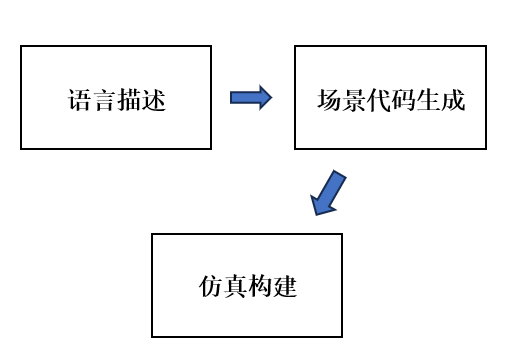
\includegraphics[width=0.8\textwidth]{"images/流程图1.pdf"}
	\caption{从自然语言描述到仿真场景构建的流程图}
	\label{fig:flowchart}
\end{figure}

本模块负责接收自然语言输入并生成对应的Scenic场景描述。具体流程如下:
输入:自然语言形式的场景描述,例如“The ego vehicle is driving on a straight road; the adversarial pedestrian suddenly appears from behind a parked car on the right front and suddenly stop.”。
检索增强:使用 \texttt{sentence-transformers} 中的 \texttt{sentence-t5-large} 模型对输入进行向量化表示,并在本地检索数据库(如 \texttt{retrieve/scenario\_descriptions.\\txt})中查找相似描述作为参考样本。
大语言模型解析:采用预训练的大语言模型(如 GPT-4o),结合检索到的参考样本,生成符合输入语义的 Scenic 脚本。
场景拼接机制:根据场景复杂度,支持对多个子元素(如车辆、行人、环境条件)进行组织与拼接。



\subsection{场景合成与仿真模块}

本模块负责将自然语言生成的Scenic脚本转化为三维可视化仿真场景,并在CARLA仿真平台上实现动态运行。整个过程包括脚本解析、场景构建、仿真控制、交互支持与数据输出等多个环节,具体如下:

	Scenic解析:本系统会先借助Scenic内置的语法与语义分析器来对输入脚本开展解析工作,Scenic作为一种领域专用语言可让用户用简洁且结构化的方式去描述场景元素像车辆、行人、障碍物等的初始状态和约束条件,解析过程能够生成涵盖对象属性如位置、速度、朝向以及交互规则如跟车距离、避让行为还有环境条件如天气、时间的完整场景配置
	
	仿真构建:完成脚本解析之后系统自动把Scenic生成中间配置映射到CARLA仿真平台里,具体涵盖载入指定地图、部署交通参与者、设定摄像头和LiDAR等传感器参数、配置天气光照路况等环境因素等内容,系统能够依据配置实现对城市道路高速公路十字路口等多种类型场景精准建模
	接口调用关系:Scenic借助和CARLA集成的Python API来调用底层仿真接口,系统会自动完成Actor的创建以及状态初始化和行为脚本绑定等任务,这极大程度简化了从脚本到仿真的转换流程,研究人员不用手动编程就能通过文本控制仿真流程,显著提升了效率和复用性。
	
	动态交互支持:系统能够支持高度动态化的场景仿真工作,还可以模拟交通参与者之间的交互行为,像车辆变道、避障、红绿灯响应以及行人横穿马路等情况,Scenic语言提供了条件触发与时间控制相关机制,允许用户描述复杂的行为序列内容,以此实现具有时序性、可演化的场景变化状况,从而增强了仿真的真实感与复杂程度。
	
	多样化仿真配置:这个模块能够支持进行灵活的仿真参数配置,其中涵盖地图选择像Town01、Town05这类,还有天气设置包含晴天、雨天、雾天等情况,以及交通流量控制和车辆控制模式如自动驾驶、手动控制等内容,这样可以满足不同的测试需求,并且该模块还支持使用不同版本的CARLA和Scenic进行组合,具备较好的兼容性与可拓展性。
	

输入数据:本实验采用约20条自然语言描述作为输入样本,用于生成自动驾驶场景。这些描述覆盖多种交通情境和突发事件,例如:

(1)自车在红绿灯前等待信号

(2)行人突然横穿街道

(3)The ego vehicle is driving on a straight road; the adversarial pedestrian appears from a driveway on the left and suddenly stop and walk diagonally.

(4)The ego vehicle is driving on a straight road when a pedestrian suddenly crosses from the right front and suddenly stops as the ego vehicle approaches.

\subsection{场景评估与展示模块}

场景评估与展示模块的目的是对生成的三维仿真场景做可视化呈现和定量分析,此模块方便研究人员直观了解场景生成具体效果,也为后续性能比较、模型调优以及系统验证提供评估依据,该模块包含下面几个关键功能:


	可视化展示:在仿真进行的过程当中系统能够自动截取关键帧的截图,或者录制完整的仿真过程视频并保存成图像或视频文件,这些可供研究人员用来做人工审阅、可视化报告展示以及用户研究评估,截图一般会选择交通事件发生点像刹车、避障、碰撞等情况,或者特定的时序节点,以此确保所展示信息具备代表性与丰富性,视频部分可以借助CARLA原生录制功能或者集成第三方渲染引擎来实现,并且支持多角度、多摄像机的可视观察,从而进一步增强场景调试与验证方面的可操作性。
	
	量化评估:本系统是在自动化生成以及仿真的基础之上,进一步引入多维度的量化评估指标,以此对场景生成的有效性、合理性和多样性进行定量测量,具体涵盖的内容有:
	
		(1)语义保真度(Semantic Fidelity):这个指标的作用是衡量输入的自然语言描述和最终生成的仿真场景之间语义一致性,可采用人工标注评分和自动化匹配算法相结合的方式来开展,比如通过设定关键语义要素像地点、交通行为、天气条件等的匹配程度,对场景是否准确还原用户意图进行评分,自动方法能够结合自然语言处理与图结构匹配技术实现初步评估进而提升效率。
		
		
		(2)多样性指标(Scene Diversity):这项指标能反映系统生成场景在多次输入不同自然语言之后的差异性以及覆盖范围,主要涵盖空间多样性像不同地图位置与道路类型等方面、元素多样性比如参与车辆行人非机动车种类情况、行为多样性包含速度控制路线选择交通交互等内容,统计方法有使用Shannon熵、Jaccard相似度或者聚类分布指标等,以此全面反映生成系统的泛化能力和表现范围。
		
		(3)驾驶性能指标(Driving Performance):为了评估生成场景对自动驾驶系统测试价值,本模块支持在生成场景里运行预设自动驾驶控制系统,像基于CARLA的自动驾驶Agent并记录其表现,关键评估维度包含碰撞率也就是单位场景中发生碰撞的比例、任务成功率即是否成功完成任务或驶出场景、路径偏离率指与理想路径的偏差程度等,这些数据能够用于评估生成场景的挑战性与安全测试覆盖度,是场景质量评估的重要依据。
	
	评估结果展示与导出:系统将展示代码运行出的评估结果用列出的形式来做可视化展示,这样方便研究人员开展对比分析以及生成结果报告,所有截图、评估指标还有分析数据都可以导出成标准格式文件,例如CSV、JSON、PNG等,可用于论文撰写、模型调试或者进一步的数据挖掘。
	






\section{系统编码与实验}